\chapter{Performance and Reliability Evaluation}\label{ch:performance}

\section{Measurement protocol}

\begin{itemize}
  \item Same database, same 23.76~million rows, same SQL text and bind values, same retention
        policy and operation order for both designs.
  \item Each query: one warm-up run and five measured runs; medians are reported. Logical reads
        (LIO), physical reads, redo, undo and CPU come from \code{V\$MYSTAT} deltas, and plans
        are saved in \code{results/plans/}.
  \item \textbf{LIO is the primary indicator.} Full scans of the 1.6~GB baseline table use
        serial direct-path reads, which bypass the buffer cache. Every baseline full scan
        therefore reads about 204\,000 blocks from disk, and its elapsed time varies with the
        laptop's I/O (from 0.5 to 2.6~s over five runs in one case). Partitions stay in cache.
        Elapsed times are client-side, so sub-millisecond queries are mostly noise.
\end{itemize}

\section{Query performance}

\begin{table}[H]
\centering\small
\caption{Workload results on the full 72-month history (before lifecycle), medians}
\label{tab:qbefore}
\begin{tabularx}{\linewidth}{lLrrrrr}
\toprule
& Query & \multicolumn{2}{c}{Elapsed (ms)} & \multicolumn{2}{c}{Logical reads} & Gain \\
& & Base & Part. & Base & Part. & time / LIO \\
\midrule
Q1 & Monthly revenue by service & 535.3 & 37.1 & 204\,092 & 3\,746 & 14$\times$ / 54$\times$ \\
Q2 & Customer history, 3 months & 0.9 & 0.8 & 6 & 12 & 1.1$\times$ / 0.5$\times$ \\
Q3 & Annual revenue 2025 & 1\,108.5 & 580.8 & 204\,092 & 39\,787 & 1.9$\times$ / 5.1$\times$ \\
Q4 & Open receivables, 6 months & 618.5 & 176.9 & 204\,092 & 21\,829 & 3.5$\times$ / 9.3$\times$ \\
Q5 & Lookup by record id & 0.6 & 0.6 & 4 & 4 & 1.0$\times$ / 1.0$\times$ \\
Q6 & Revenue per year, no filter & 2\,623.3 & 2\,750.7 & 204\,092 & 204\,158 & 1.0$\times$ / 1.0$\times$ \\
Q7 & Disputes in March 2022 & 1\,410.7 & 13.0 & 204\,108 & 2\,369 & 109$\times$ / 86$\times$ \\
\bottomrule
\end{tabularx}
\end{table}

\begin{table}[H]
\centering\small
\caption{Workload results after the retention policy (Q7 through the online + archive views)}
\label{tab:qafter}
\begin{tabularx}{\linewidth}{lLrrrrr}
\toprule
& Query & \multicolumn{2}{c}{Elapsed (ms)} & \multicolumn{2}{c}{Logical reads} & Gain \\
& & Base & Part. & Base & Part. & time / LIO \\
\midrule
Q1 & Monthly revenue by service & 534.1 & 39.5 & 211\,566 & 3\,746 & 14$\times$ / 56$\times$ \\
Q2 & Customer history, 3 months & 1.2 & 0.8 & 6 & 12 & 1.5$\times$ / 0.5$\times$ \\
Q3 & Annual revenue 2025 & 978.9 & 664.3 & 211\,566 & 30\,338 & 1.5$\times$ / 7.0$\times$ \\
Q4 & Open receivables, 6 months & 595.2 & 174.8 & 211\,566 & 21\,829 & 3.4$\times$ / 9.7$\times$ \\
Q5 & Lookup by record id & 0.4 & 0.4 & 4 & 4 & 1.0$\times$ / 1.0$\times$ \\
Q6 & Revenue per year, no filter & 2\,089.7 & 1\,636.2 & 211\,566 & 103\,677 & 1.3$\times$ / 2.0$\times$ \\
Q7 & Disputes in March 2022 & 383.0 & 8.9 & 163\,098 & 1\,690 & 43$\times$ / 97$\times$ \\
\bottomrule
\end{tabularx}
\end{table}

\begin{figure}[H]
  \centering
  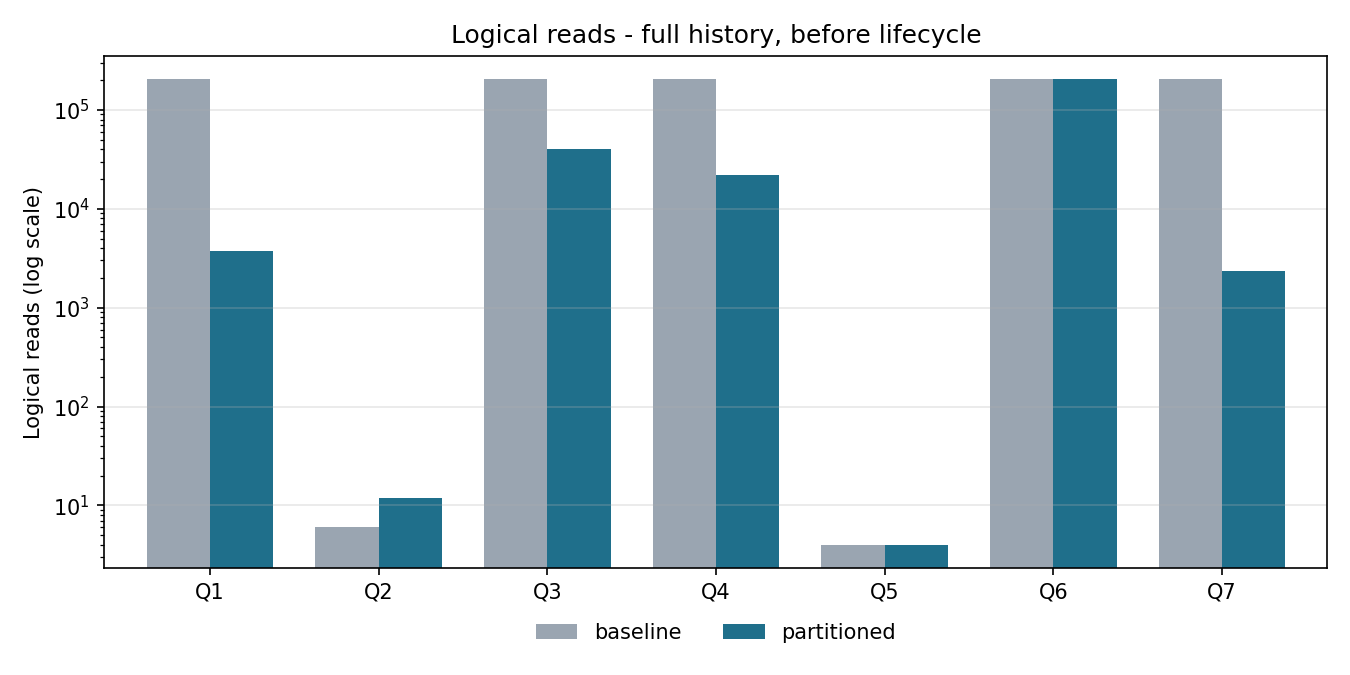
\includegraphics[width=0.92\linewidth]{queries_before_lio}
  \caption{Logical reads per query on the full history (log scale)}
  \label{fig:lio}
\end{figure}

\paragraph{Interpretation.}
\begin{itemize}
  \item \textbf{Date-bounded reports} (Q1, Q4, Q7) gain the most, because partition pruning
        reads only the requested months. The baseline full-scans the table, since a single
        month is too large a share of the rows for its \code{bill\_date} index.
  \item \textbf{Q3} reads 5--7 times fewer blocks but runs only 1.5--1.9 times faster. It
        aggregates about 4.6~million rows, so CPU dominates once I/O is gone. After the
        lifecycle, 10 of its 12 months are compressed, and decompression costs CPU.
  \item \textbf{Q6 has no date predicate}, so nothing can be pruned. Partitioning is not a
        universal accelerator. After the lifecycle Q6 reads half the blocks, because the
        online table holds 38 months, 24 of them compressed.
  \item \textbf{OLTP lookups} are unchanged in time. Q5 uses the global primary key in both
        designs. Q2 reads 12 blocks instead of 6, because the local index has one B-tree per
        month and the query covers three months. This is the cost of local indexes, and it is
        negligible here.
\end{itemize}

\begin{figure}[H]
  \centering
  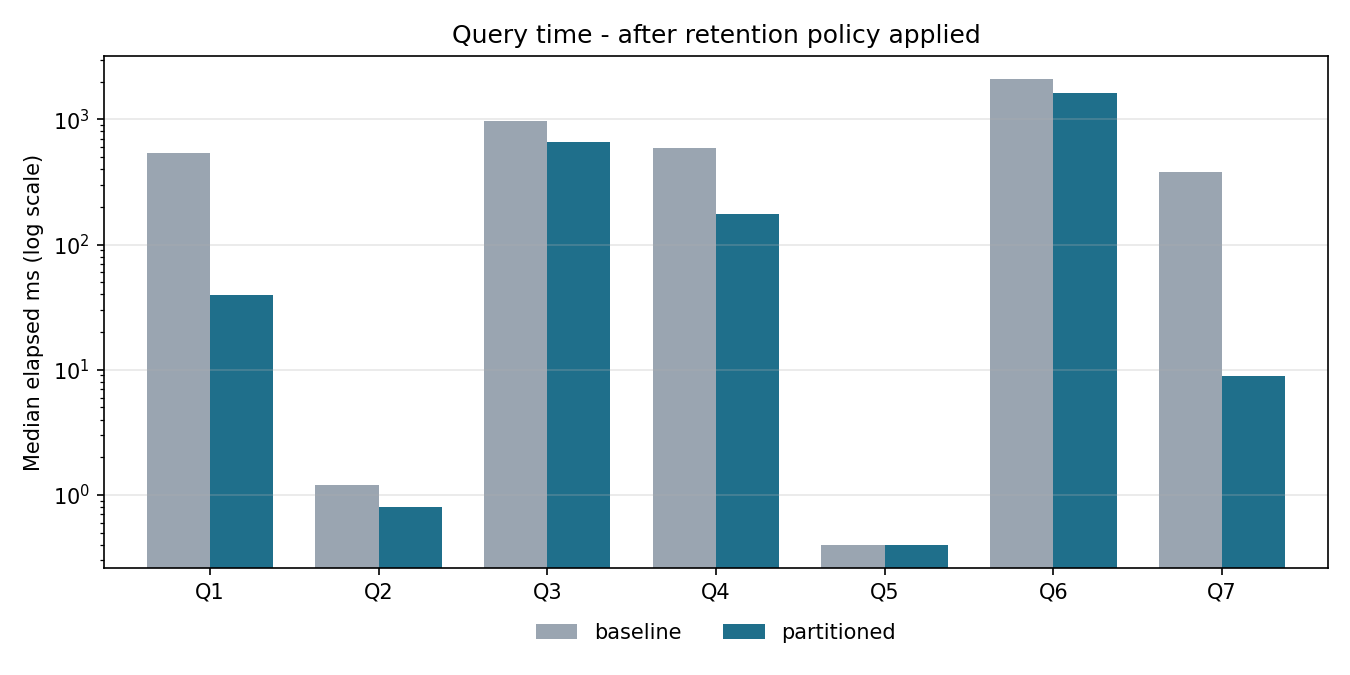
\includegraphics[width=0.92\linewidth]{queries_after_time}
  \caption{Median elapsed time per query after the retention policy (log scale)}
  \label{fig:qafter}
\end{figure}

\section{Maintenance operations}

The lifecycle was applied in steady-state order: the oldest months were warmed and archived
first, then purged \emph{from the archive}, exactly as they would be after two years in the
archive. Both designs followed this order.

\begin{table}[H]
\centering\small
\caption{Maintenance cost per operation (averages)}
\label{tab:maint}
\begin{tabularx}{\linewidth}{Lrrrrl}
\toprule
Operation (one month) & \multicolumn{2}{c}{Seconds} & \multicolumn{2}{c}{Redo (MB)} & Gain \\
& Base & Part. & Base & Part. & time \\
\midrule
Archive & 26.17 & 0.42 & 498.8 & 6.3 & 62$\times$ \\
Purge & 5.14 & 0.02 & 110.0 & $<$0.1 & $\approx$250$\times$ \\
Warm (freeze, move, compress) & -- & 3.06 & -- & 152.9 & new step \\
\textbf{Monthly job} & \textbf{31.31} & \textbf{3.51} & \textbf{608.8} & \textbf{159.3} & \textbf{8.9$\times$} \\
Load one month (429\,000 rows) & 4.36 & 2.13 & 101.9 & 76.1 & 2.0$\times$ \\
Statistics, routine refresh & 35.44 & 14.44 & 5.7 & 2.6 & 2.5$\times$ \\
Statistics, first after migration & 32.21 & 75.27 & 5.6 & 94.3 & 0.4$\times$ \\
\bottomrule
\end{tabularx}
\end{table}

The \emph{monthly job} is the fair steady-state comparison. In the baseline it is one archive
and one purge. In the partitioned design it is one warm, one archive and one purge, because
the zero-copy archive relies on the month having been compressed by the warm step. It is
8.9 times faster, with 3.8 times less redo and 4.0 times less undo. Applying the whole policy
to the six-year history at once took 1\,004~s and 19.3~GB of redo for the baseline, against
199~s and 9.4~GB for the partitioned design. Of the partitioned figures, 184~s and 9.2~GB are
the one-time warm catch-up of 60 months.

\begin{figure}[H]
  \centering
  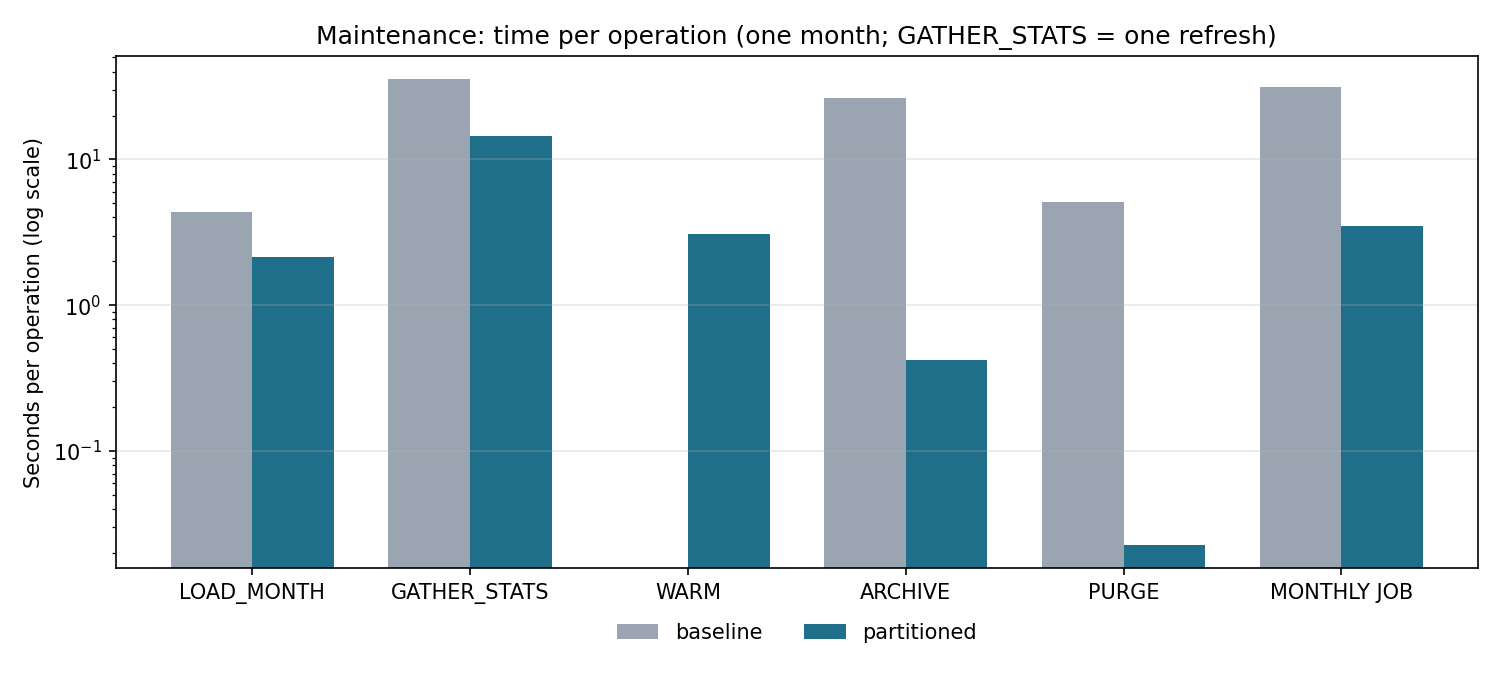
\includegraphics[width=0.95\linewidth]{maintenance_time}
  \caption{Maintenance time per operation (log scale)}
  \label{fig:maint}
\end{figure}

\paragraph{Interpretation.}
\begin{itemize}
  \item Archive and purge become metadata operations: their cost no longer depends on the
        number of rows. The baseline's \code{DELETE}s generate undo and redo for every row and
        every index entry. In ARCHIVELOG mode (production) this redo would also have to be
        archived, backed up and shipped to a standby.
  \item \textbf{WARM is the main cost of the new design} (3.1~s and 153~MB of redo per month).
        It moves and compresses the month, maintains the global primary key, rebuilds the
        local index partition and re-captures the control totals. We did not measure these
        parts separately; global index maintenance is the likely main part.
  \item The \textbf{first statistics refresh after the migration} re-analysed all 73
        partitions (75~s). The next routine refresh re-analysed only the new partition (14~s,
        2.5 times faster than the baseline). This is a one-time cost of the migration.
\end{itemize}

\section{Storage}

\begin{table}[H]
\centering
\caption{Space used, tables and their indexes (MB)}
\label{tab:space}
\begin{tabular}{lrr}
\toprule
Table & Before & After policy \\
\midrule
Baseline online (\code{BILLING\_RECORDS\_BASE}) & 3\,152 & 3\,248 \\
Baseline archive (\code{BILLING\_ARCHIVE\_BASE}, 2 indexes) & 0 & 1\,304 \\
Partitioned online (\code{BILLING\_RECORDS}) & 3\,121 & 1\,975 \\
Partitioned archive (\code{BILLING\_ARCHIVE}, 1 local index) & 0 & 587 \\
\midrule
\textbf{Retained data, baseline / partitioned} & & \textbf{4\,552 / 2\,562 (-44\,\%)} \\
\bottomrule
\end{tabular}
\end{table}

After 36 of its 74 months were moved out, the baseline table did not shrink. It even grew,
because new months were loaded above the high-water mark, and full scans still read about
212\,000 blocks. The baseline archive also keeps the space of the months deleted from it.
Releasing that space would require \code{SHRINK SPACE} or \code{MOVE} on large tables. With
partitions, a purge releases space immediately and BASIC compression shrinks warm and
archived months. The archive comparison combines compression, one index fewer and the space
the baseline did not release.

\section{Integrity and reliability}

After the whole benchmark, \textbf{62 of 62} retained months match their control totals in
both designs (row count, amount total and fingerprint sum), and every purged month is absent.
Together with the functional tests (crash and resume, interrupted warm, deliberate
corruption detected) this supports the reliability indicators K8 and K9.

\section{Indicators against targets}

\begin{longtable}{lp{0.3\linewidth}p{0.36\linewidth}l}
\caption{KPI results}\label{tab:kpiresults}\\
\toprule
KPI & Target & Result & Status \\
\midrule
\endfirsthead
\toprule
KPI & Target & Result & Status \\
\midrule
\endhead
K1 & $\geq$5$\times$ time, $\geq$10$\times$ LIO & 14$\times$ / 54--56$\times$ & met \\
K2 & $\geq$5$\times$ fewer LIO & 86$\times$ before, 97$\times$ after & met \\
K3 & no time regression $>$2$\times$ & Q5 unchanged; Q2 0.9 $\rightarrow$ 0.8~ms & met \\
K4 & archive $\geq$10$\times$, $<$5~s & archive operation 62$\times$, 0.42~s; whole monthly job 8.9$\times$, 3.5~s & met / \textbf{partly} \\
K5 & purge $<$1~s & 0.02~s & met \\
K6 & load + stats not slower & 2.0$\times$ and 2.5$\times$ faster (first gather slower, once) & met \\
K7 & $\geq$25\,\% less storage & $-$44\,\% & met \\
K8 & 100\,\% integrity & 62/62 months, both designs & met \\
K9 & 0 rows lost, re-run recovers & T12--T17, T41, Scenario 4 & met \\
K10 & 100\,\% security checks & 25/25 & met \\
K11 & one command per month & \code{dlm\_pkg.run\_lifecycle} & met \\
\bottomrule
\end{longtable}

Ten indicators are met. K4 is met for the archive operation itself (62 times faster). When
the warm step that the archive depends on is included, the whole monthly job is 8.9 times
faster, just under the 10$\times$ target. Section~\ref{sec:improvements} discusses how to
reduce the warm cost.
